\documentclass[12pt,a4paper]{article}
\usepackage[utf8]{inputenc}
\usepackage[T1]{fontenc}
\usepackage{amsmath,amssymb,amsfonts}
\usepackage{graphicx}
\usepackage{booktabs}
\usepackage{longtable}
\usepackage{hyperref}
\usepackage{listings}
\usepackage{xcolor}
\usepackage{algorithm}
\usepackage{algpseudocode}
\usepackage{tikz}
\usetikzlibrary{shapes,arrows,positioning,fit}
\usepackage{float}
\usepackage{subcaption}
\usepackage{geometry}
\geometry{margin=1in}
\usepackage{setspace}
\onehalfspacing

% Code listing style
\lstset{
    basicstyle=\ttfamily\small,
    breaklines=true,
    frame=single,
    numbers=left,
    numberstyle=\tiny\color{gray},
    keywordstyle=\color{blue},
    commentstyle=\color{green!60!black},
    stringstyle=\color{red},
    backgroundcolor=\color{gray!10}
}

\title{\textbf{Automated Incident Response Using Deep Reinforcement Learning}\\
\large A Comprehensive Technical Report}
\author{
\begin{tabular}{ll}
Pratyush Kumar & 23BCS099 \\
Ritik Kumar Shahi & 23BCS110 \\
Saisha Bore & 23BCS116 \\
Aryan Talikoti & 23BCS018 \\
\end{tabular}
}
\date{January 2026}

\newcommand{\projecturl}{\url{https://github.com/pratyushKr04/automated-incident-response-using-RL.git}}

\begin{document}

\maketitle

\begin{abstract}
In this report, we describe our work on applying Deep Reinforcement Learning (DRL) to automate incident response in cybersecurity. Building on the approach of Hammar and Stadler \cite{hammar2021}, who showed that DQN variants can learn effective security strategies in simulated network environments, we developed a custom Gymnasium environment that realistically mimics attack scenarios---specifically brute force and ransomware---using parameters extracted from the CICIDS 2017 and CERT Insider Threat datasets. Our agent is a Deep Q-Network (DQN) that uses both the Dueling architecture and Double DQN, and it learns defensive strategies by interacting with this simulated environment over many episodes. Through our experiments, we found that the DRL agent outperforms several traditional rule-based approaches, including baselines inspired by Snort, NIST 800-61, and MITRE ATT\&CK pattern matching. We ran independent samples t-tests, computed Cohen's d effect sizes, and constructed 95\% confidence intervals to check statistical significance. The agent ends up with a 75\% success rate, with statistically significant gains over every baseline we tested (p < 0.05). Against the random baseline, Cohen's d came out to 5.55, and against the threshold-based approach it was 0.35.
\end{abstract}

\tableofcontents
\newpage

%==============================================================================
\section{Introduction}
%==============================================================================

\subsection{Background and Motivation}

Over the last decade or so, the cybersecurity landscape has changed quite a bit. Organizations today face threats that would have been hard to imagine just a few years ago, and the pace at which new attack methods appear keeps accelerating. Traditional cybersecurity tools---things like Security Information and Event Management (SIEM) systems and Intrusion Detection Systems (IDS)---are still fundamental to enterprise security, but they have some real limitations. Most of them rely on known patterns and signatures, which means they can struggle with novel or evolving attacks that don't match anything in their databases.

But the challenge goes beyond just detection. When an alert fires, a human analyst has to sift through potentially hundreds of notifications, many of which turn out to be false alarms, and then decide what to do about the real ones. This needs to happen fast---modern attacks can spread through a network in minutes. The sheer volume of alerts and the speed required to respond make a pretty compelling argument for some form of intelligent automation.

Machine learning has already shown promise in several areas of cybersecurity, from classifying malware to spotting anomalies in network traffic. That said, most of those applications treat each observation independently. Incident response is different: it's a sequential decision problem where each action you take changes what happens next. If you block an IP address now, the attacker might pivot to a different entry point. If you wait too long, they might already be inside. This sequential nature is exactly what reinforcement learning is designed to handle. Recent work by Hammar and Stadler \cite{hammar2021} demonstrated that DQN-based agents---including Double DQN and Dueling DQN variants---can learn effective cyber defense strategies through self-play in simulated enterprise networks. Their results were a big motivation for us to try a similar approach but applied specifically to incident response, with attack simulations grounded in real-world datasets.

So the goal of this project was to explore whether Deep Reinforcement Learning could be used to build an incident response system that learns good defensive strategies on its own, just by interacting with a simulated environment. Taking inspiration from \cite{hammar2021}, we frame the problem as a Markov Decision Process and use DQN variants to let the agent pick up on temporal patterns and develop strategies over time rather than just reacting to individual data points.

\subsection{Problem Statement}

At its core, what we're trying to do is build an agent that can make sensible incident response decisions based solely on observable system metrics. The agent gets a continuous stream of data---login attempt rates, file access patterns, CPU usage---and has to figure out what's going on and what to do about it.

More specifically, the agent needs to: detect attacks from inherently noisy observations (the real world is messy, after all); pick the right defensive action from a set of options; avoid jumping at shadows and creating false positives that disrupt normal operations; and ideally, generalize what it learns so it can handle different types of attacks without us having to hard-code detection rules for each one.

This is tricky for a few reasons. The observations the agent gets are noisy---they're rough approximations of what's actually happening in the system, similar to what a real security tool would see. On top of that, the consequences of an action aren't always immediately obvious. If the agent responds too early, it might be a false positive. If it waits too long, the attacker could be already in. There's a real tension between being aggressive (and risking unnecessary disruptions) and being cautious (and risking a successful breach).

%==============================================================================
\section{Related Work}
%==============================================================================

\subsection{Intrusion Detection Systems}

Intrusion detection has been around for decades at this point, and the systems generally fall into two camps: signature-based and anomaly-based. Signature-based IDS, like Snort, keep a database of known attack patterns and try to match incoming traffic against those patterns. They're great at catching known threats and tend to have low false positive rates, but they're fundamentally reactive---if nobody has written a signature for an attack, the system won't catch it. Keeping those signature databases up to date is a constant headache, and zero-day exploits slip right through.

Anomaly-based systems take the opposite approach: they build up a picture of what ``normal'' looks like and then flag anything that deviates from that baseline. In theory, this lets them catch attacks nobody has seen before. In practice, though, they tend to generate a lot of false alarms, because legitimate behavior varies quite a bit day to day. It's also not easy to pin down what ``normal'' even means in a dynamic environment, and clever attackers can sometimes evade detection by changing their behavior gradually. Balancing detection sensitivity against false alarm rates is still one of the central problems in this area.

\subsection{Machine Learning in Cybersecurity}

Machine learning has found a lot of applications in cybersecurity over recent years. Random Forests and SVMs have been used for network intrusion detection, usually working with features pulled from packet headers and flow data. Deep neural networks have done well at malware classification, where they can learn useful representations from raw binaries or behavioral logs.

Autoencoders are particularly interesting for anomaly detection because they're unsupervised---they learn what ``normal'' looks like by compressing and reconstructing normal data, and then anything that doesn't reconstruct well gets flagged. This sidesteps the perennial problem of not having enough labeled attack data for training. RNNs and LSTMs have also been applied to sequence-based detection tasks, where you need to pick up on temporal patterns in network traffic or system call sequences that might indicate a multi-stage attack unfolding over time.

All that said, most of these approaches are essentially classifiers or anomaly detectors. They look at individual observations (or short sequences) and say ``attack'' or ``not attack.'' They don't really address the question of what you should \textit{do} about a detected threat, or how to balance competing goals---like minimizing response time versus avoiding false positives---over a sequence of decisions. That's the gap we're trying to fill.

\subsection{Reinforcement Learning for Security}

Reinforcement learning is a natural fit for problems where you need to make a sequence of decisions under uncertainty, and where each decision affects what comes next. Several groups have applied RL to security-related tasks: autonomous penetration testing (training agents to find vulnerabilities in simulated networks), adaptive honeypot configuration (learning what fake services to present to maximize intelligence gathering), and network defense games where the defender and attacker are modeled as adversaries in a game-theoretic setting.

The work closest to ours is by Hammar and Stadler \cite{hammar2021}, who trained autonomous cyber-defense agents using DQN, Double DQN, and Dueling DQN in simulated enterprise networks provided by Microsoft's CyberBattleSim. They modeled the interaction between attackers and defenders as a Markov game and showed that off-policy deep RL algorithms can learn effective security strategies through self-play. Their results were promising---the trained agents outperformed heuristic baselines---but the focus was on network-level attack and defense rather than on the incident response decision-making that security analysts face day to day.

Our work builds on their approach but takes it in a somewhat different direction. We're focused specifically on the incident response decision---given that something suspicious might be happening, what should the system actually do? Rather than using a pre-built simulation platform, we built a custom Gymnasium environment with attack simulations grounded in real data (from the CICIDS 2017 and CERT datasets), and we compare against baselines inspired by established security frameworks like Snort, NIST 800-61, and MITRE ATT\&CK. We think this adds some practical grounding that complements the more abstract game-theoretic perspective in \cite{hammar2021}.

\subsection{Security Frameworks and Standards}

For our baselines, we drew from three well-known security resources. Snort is an open-source IDS/IPS that uses signature matching and protocol analysis---it's probably the most widely used open-source IDS out there. NIST SP 800-61 is the government's guide for computer security incident handling, and it lays out a structured approach to categorizing and responding to incidents. The MITRE ATT\&CK framework organizes known adversary tactics and techniques into a structured knowledge base that a lot of security teams use for detection and response planning.

%==============================================================================
\section{Methodology}
%==============================================================================

\subsection{System Architecture}

Following the general approach established by Hammar and Stadler \cite{hammar2021} for training RL agents in security environments, our system follows the standard RL setup: an agent interacts with an environment in a loop of observation, action, and reward. At each timestep, the environment hands the agent a 9-dimensional state vector describing the current situation. The agent---a Dueling Double DQN, chosen because \cite{hammar2021} showed these variants outperform vanilla DQN for security tasks---processes this through a neural network to estimate how good each possible action is, then picks an action using an epsilon-greedy policy. The environment responds by updating the attack state, calculating a reward, and producing the next observation.

We kept the design modular on purpose. The attack simulator handles the state transitions and generates the observable metrics; the environment wrapper implements the Gymnasium interface and computes rewards; and the agent module contains the neural network, experience replay buffer, and learning algorithm. Splitting things up this way made it a lot easier to experiment with different attack types, reward structures, and so on without having to rewrite everything each time.

\begin{figure}[H]
\centering
\resizebox{\textwidth}{!}{%
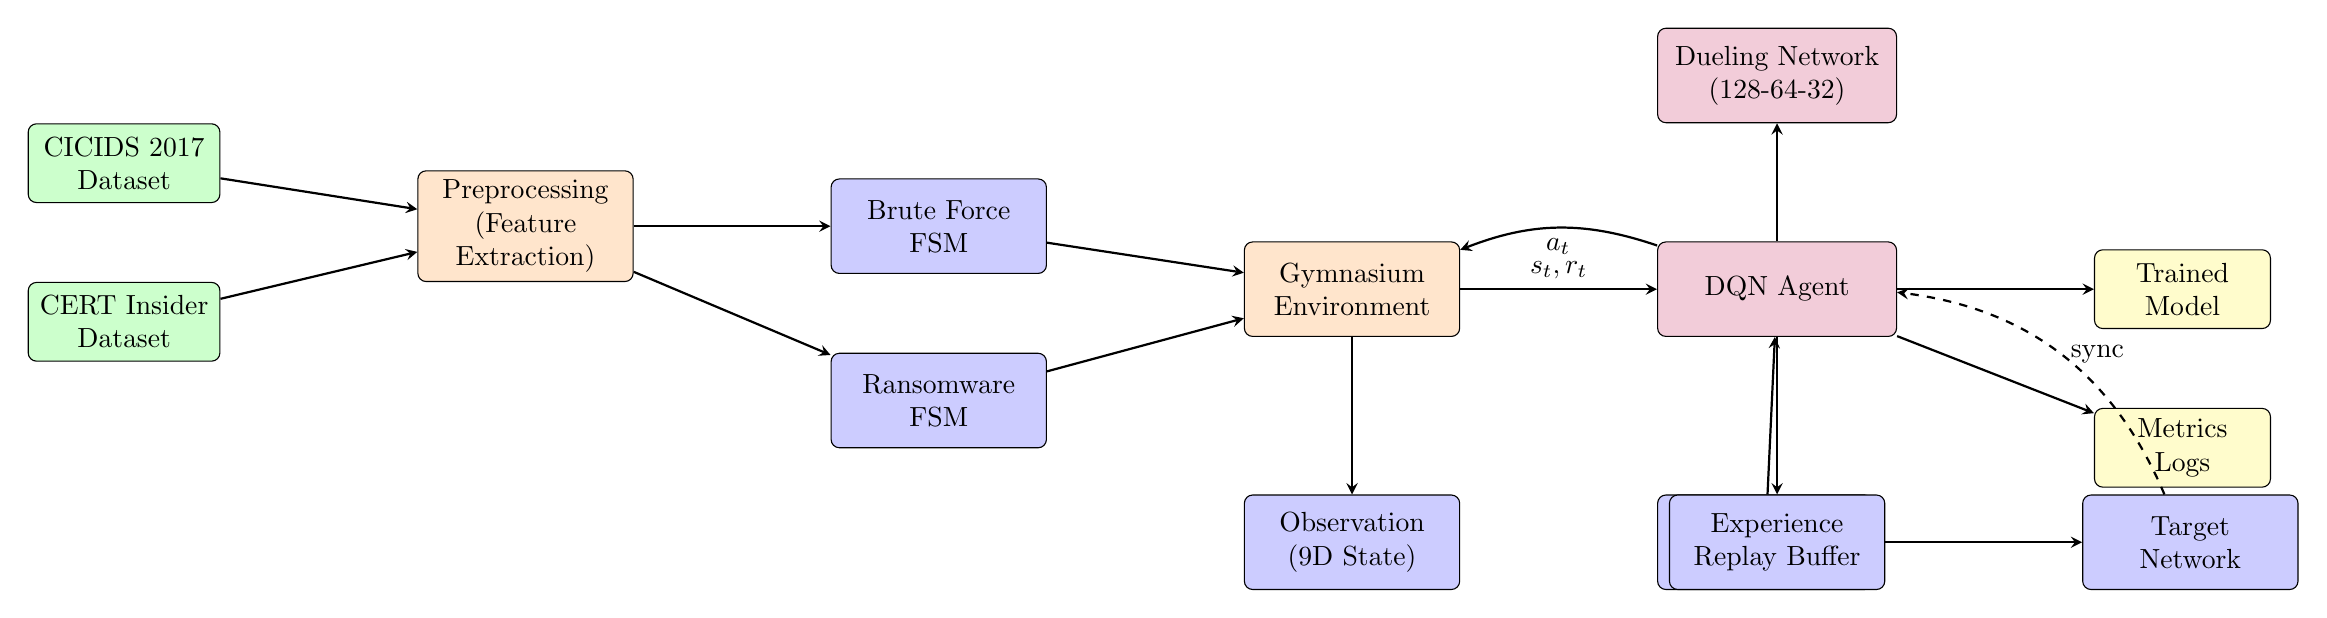
\begin{tikzpicture}[
    node distance=1.8cm and 2.5cm,
    block/.style={rectangle, draw, fill=blue!20, text width=2.5cm, text centered, minimum height=1.2cm, rounded corners=3pt},
    data/.style={rectangle, draw, fill=green!20, text width=2.2cm, text centered, minimum height=1cm, rounded corners=3pt},
    process/.style={rectangle, draw, fill=orange!20, text width=2.5cm, text centered, minimum height=1.2cm, rounded corners=3pt},
    network/.style={rectangle, draw, fill=purple!20, text width=2.8cm, text centered, minimum height=1.2cm, rounded corners=3pt},
    output/.style={rectangle, draw, fill=yellow!20, text width=2cm, text centered, minimum height=1cm, rounded corners=3pt},
    arrow/.style={thick,->,>=stealth},
    dasharrow/.style={thick,->,>=stealth,dashed}
]
    % Data Sources
    \node[data] (cicids) {CICIDS 2017\\Dataset};
    \node[data, below=1cm of cicids] (cert) {CERT Insider\\Dataset};
    
    % Preprocessing
    \node[process, right=2.5cm of cicids, yshift=-0.8cm] (preprocess) {Preprocessing\\(Feature Extraction)};
    
    % Attack Simulators
    \node[block, right=2.5cm of preprocess] (bruteforce) {Brute Force\\FSM};
    \node[block, below=1cm of bruteforce] (ransomware) {Ransomware\\FSM};
    
    % Environment
    \node[process, right=2.5cm of bruteforce, yshift=-0.8cm] (env) {Gymnasium\\Environment};
    
    % Observation/Action
    \node[block, below=2cm of env] (obs) {Observation\\(9D State)};
    \node[block, right=2.5cm of obs] (action) {Action\\(5 Options)};
    
    % DQN Agent
    \node[network, right=2.5cm of env] (agent) {DQN Agent};
    
    % Neural Network Details
    \node[network, above=1.5cm of agent] (nn) {Dueling Network\\(128-64-32)};
    
    % Training Components
    \node[block, below=2cm of agent] (replay) {Experience\\Replay Buffer};
    \node[block, right=2.5cm of replay] (target) {Target\\Network};
    
    % Outputs
    \node[output, right=2.5cm of agent] (model) {Trained\\Model};
    \node[output, below=1cm of model] (logs) {Metrics\\Logs};
    
    % Arrows - Data Flow
    \draw[arrow] (cicids) -- (preprocess);
    \draw[arrow] (cert) -- (preprocess);
    \draw[arrow] (preprocess) -- (bruteforce);
    \draw[arrow] (preprocess) -- (ransomware);
    \draw[arrow] (bruteforce) -- (env);
    \draw[arrow] (ransomware) -- (env);
    
    % RL Loop
    \draw[arrow] (env) -- node[above] {$s_t, r_t$} (agent);
    \draw[arrow] (agent) to[bend right=20] node[below] {$a_t$} (env);
    \draw[arrow] (env) -- (obs);
    \draw[arrow] (action) -- (agent);
    
    % Training Flow
    \draw[arrow] (agent) -- (nn);
    \draw[arrow] (agent) -- (replay);
    \draw[arrow] (replay) -- (target);
    \draw[dasharrow] (target) to[bend right=30] node[right] {sync} (agent);
    
    % Outputs
    \draw[arrow] (agent) -- (model);
    \draw[arrow] (agent) -- (logs);
    
\end{tikzpicture}%
}
\caption{Complete system architecture showing data flow from datasets through preprocessing, attack simulation, environment interaction, DQN agent with Dueling network architecture, and training outputs.}
\label{fig:architecture}
\end{figure}

\subsection{Custom Gymnasium Environment}

We implemented our environment using the standard Gymnasium API, which means it plugs into most existing RL libraries without any fuss. The observation space is a continuous 9-dimensional box and the action space has five discrete options. Each episode runs for up to 100 timesteps---think of it as a monitoring window where attacks may or may not happen, and the agent has to decide how to respond.

We put some thought into what the observation space should look like, trying to include the kinds of information that a real automated security system would reasonably have access to. The raw metrics are login attempt rate, file access rate, and CPU utilization. On top of these, we added some derived features: rate-of-change values for each metric (to catch sudden spikes when an attack kicks off), moving averages over a 10-step window (to smooth out noise and highlight patterns that persist over time), and a sustained anomaly indicator that tracks how long the metrics have been elevated (to help tell apart a brief legitimate spike from an ongoing attack).

For actions, the agent can choose from five responses, going from least to most aggressive. ``Do nothing'' means keep watching---appropriate when things look normal. ``Block IP'' cuts off traffic from a suspicious source. ``Lock account'' freezes a potentially compromised user account. ``Terminate process'' kills suspicious running processes. And ``isolate host,'' the nuclear option, quarantines an entire machine from the network. Each of these carries different costs and has different effectiveness depending on what kind of attack is happening and how far it has progressed.

\begin{table}[H]
\centering
\caption{Action Space Definition}
\begin{tabular}{clp{6cm}}
\toprule
\textbf{Index} & \textbf{Action} & \textbf{Description} \\
\midrule
0 & do\_nothing & Continue monitoring without intervention \\
1 & block\_ip & Block the source IP address \\
2 & lock\_account & Lock the targeted user account \\
3 & terminate\_process & Kill suspicious processes \\
4 & isolate\_host & Quarantine the entire host \\
\bottomrule
\end{tabular}
\end{table}

\subsection{Attack Simulator Design}

We model attacks as Finite State Machines (FSMs) with probabilistic transitions between states. This reflects how real attacks tend to work---they don't just happen all at once but progress through phases, from initial probing to active exploitation to eventual compromise. And importantly, defensive actions can interrupt this progression, with the probability of success depending on both the attack stage and the specific action taken.

For the brute force simulator, we're modeling SSH credential stuffing. The system starts in an idle state with normal baseline metrics. At each timestep, there's a 0.15 probability that an attack begins and the system moves to a probing state, where the attacker is scanning for vulnerable accounts and the metrics tick up a bit. From probing, there's a 0.2 chance per timestep of escalating to active---this is the heavy-duty login attempt phase. Finally, from active, there's a 0.15 probability of reaching the compromised state, meaning the attacker got in. Once compromised, the episode ends with a big penalty.

The ransomware simulator works similarly but with different phases. It starts with execution (malware running, CPU spikes), moves to encryption (file access rates go through the roof as files get encrypted), and ends with data\_loss (encryption complete, ransom note deployed). We calibrated the transition probabilities and the observable metric distributions using patterns from the CICIDS 2017 and CERT datasets, so the numbers aren't just made up---they reflect what these attacks actually look like in terms of system behavior.

\begin{figure}[H]
\centering
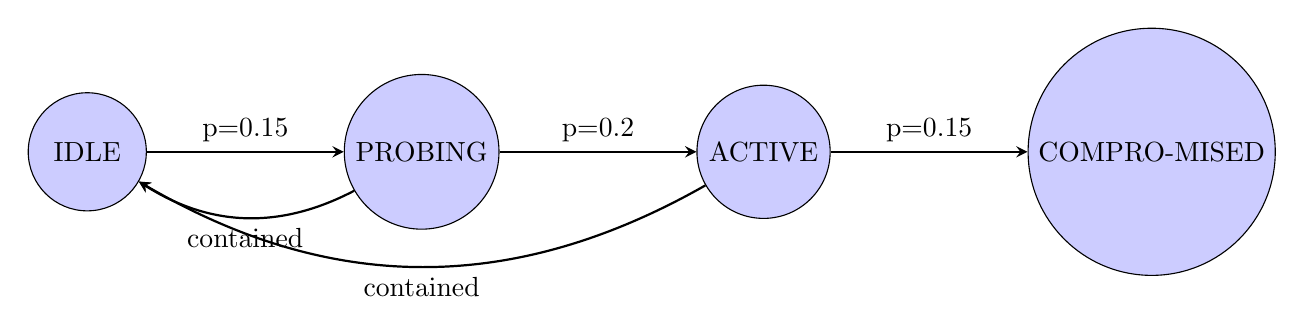
\begin{tikzpicture}[
    node distance=2.5cm,
    state/.style={circle, draw, fill=blue!20, minimum size=1.5cm},
    arrow/.style={thick,->,>=stealth}
]
    \node[state] (idle) {IDLE};
    \node[state, right=of idle] (probe) {PROBING};
    \node[state, right=of probe] (active) {ACTIVE};
    \node[state, right=of active] (comp) {COMPRO-\\MISED};
    
    \draw[arrow] (idle) -- node[above] {p=0.15} (probe);
    \draw[arrow] (probe) -- node[above] {p=0.2} (active);
    \draw[arrow] (active) -- node[above] {p=0.15} (comp);
    
    \draw[arrow, bend left=30] (probe) to node[below] {contained} (idle);
    \draw[arrow, bend left=30] (active) to node[below] {contained} (idle);
\end{tikzpicture}
\caption{Brute Force Attack Finite State Machine showing states and transition probabilities.}
\label{fig:bruteforce_fsm}
\end{figure}

\begin{table}[H]
\centering
\caption{Brute Force Observable Metrics}
\begin{tabular}{lccc}
\toprule
\textbf{State} & \textbf{Login Rate} & \textbf{File Rate} & \textbf{CPU \%} \\
\midrule
IDLE & $\sim$Poisson(5) & $\sim$Poisson(10) & $\sim$N(30, 5) \\
PROBING & $\sim$Poisson(15) & $\sim$Poisson(15) & $\sim$N(40, 5) \\
ACTIVE & $\sim$Poisson(50) & $\sim$Poisson(20) & $\sim$N(60, 10) \\
COMPROMISED & $\sim$Poisson(100) & $\sim$Poisson(50) & $\sim$N(80, 10) \\
\bottomrule
\end{tabular}
\end{table}

\begin{table}[H]
\centering
\caption{Ransomware Observable Metrics}
\begin{tabular}{lccc}
\toprule
\textbf{State} & \textbf{Login Rate} & \textbf{File Rate} & \textbf{CPU \%} \\
\midrule
IDLE & $\sim$Poisson(5) & $\sim$Poisson(10) & $\sim$N(30, 5) \\
EXECUTION & $\sim$Poisson(5) & $\sim$Poisson(30) & $\sim$N(70, 10) \\
ENCRYPTION & $\sim$Poisson(5) & $\sim$Poisson(150) & $\sim$N(90, 5) \\
DATA\_LOSS & $\sim$Poisson(10) & $\sim$Poisson(200) & $\sim$N(95, 3) \\
\bottomrule
\end{tabular}
\end{table}

One thing worth noting is that defensive actions don't always work---their effectiveness is probabilistic and depends on the attack stage. Blocking an IP address, for example, works about 90\% of the time during probing, but only 30\% of the time after the system is already compromised (by that point the attacker might have established multiple access paths). Host isolation stays effective across all stages, but it's expensive operationally. This creates the kind of tradeoffs we want the agent to learn---the more aggressive the response, the more likely it is to work, but also the more costly if it turns out to be unnecessary.

\subsection{Reward Function Design}

Getting the reward function right was one of the trickier parts of this project, since it has to capture what we actually want the agent to optimize for. We want it to contain attacks quickly, but we also don't want it overreacting to every blip in the metrics.

Here's what we settled on: catching an attack early (during stages 0--1) gets the biggest reward at +50, because that's the ideal outcome. Catching it later (stage 2+) still gets +20---late containment is better than no containment. Correctly choosing to do nothing when things are actually fine earns a small +1, which teaches the agent to be patient and not swing at everything.

On the penalty side, false positives cost $-10$. This reflects the real-world cost of shutting things down unnecessarily---if you lock someone's account for no reason, that's a problem. Missing an attack entirely that leads to compromise is $-30$, the harshest penalty (besides the accumulated step costs). We also added a $-5$ penalty for redundant actions, like blocking the same IP twice, and a tiny $-0.1$ per-step cost to create some time pressure so the agent doesn't just sit around indefinitely.

\begin{table}[H]
\centering
\caption{Reward Structure}
\begin{tabular}{lrl}
\toprule
\textbf{Event} & \textbf{Reward} & \textbf{Rationale} \\
\midrule
Early containment (stage 0-1) & +50.0 & Encourage quick response \\
Late containment (stage 2+) & +20.0 & Still valuable \\
Correct no-action & +1.0 & Reward patience \\
False positive & -10.0 & Penalize over-reaction \\
Missed attack (compromised) & -30.0 & Penalize missed threats \\
Unnecessary action & -5.0 & Penalize redundancy \\
Step penalty & -0.1 & Time pressure \\
\bottomrule
\end{tabular}
\end{table}

\subsection{DQN Agent Architecture}

Our agent uses Deep Q-Learning with two enhancements that we found made a noticeable difference: Double DQN and the Dueling architecture.

The problem with vanilla DQN is that it uses the same network to both pick the best action and estimate how good that action is. This leads to a well-known overestimation problem---the network tends to be overly optimistic about Q-values. Double DQN fixes this by splitting the two jobs: the online network picks the action it thinks is best, but the target network evaluates how good that action actually is. It's a simple change but it makes training noticeably more stable.

The Dueling architecture is the other piece. Instead of having the network directly output a Q-value for each action, we split the computation into two streams: one that estimates the value of being in a given state ($V(s)$), and another that estimates how much better or worse each action is compared to the average ($A(s,a)$). These combine as $Q(s,a) = V(s) + (A(s,a) - \text{mean}(A))$, with the mean subtraction making the decomposition identifiable. The intuition here is that in many states, the action you pick doesn't matter much (e.g., if everything is clearly fine, ``do nothing'' is obviously correct regardless of the details). The dueling structure lets the network learn that some states are just good or bad without having to figure out the value of every individual action in those states.

For the actual network, we have shared hidden layers with 128 and 64 units (ReLU activations), and then the two streams each add a 32-unit layer. The value stream ends in a single output and the advantage stream produces five outputs (one per action). We used Adam with a learning rate of 0.001, and the target network gets synced with the online network every 10 episodes.

\begin{figure}[H]
\centering
\resizebox{0.85\textwidth}{!}{%
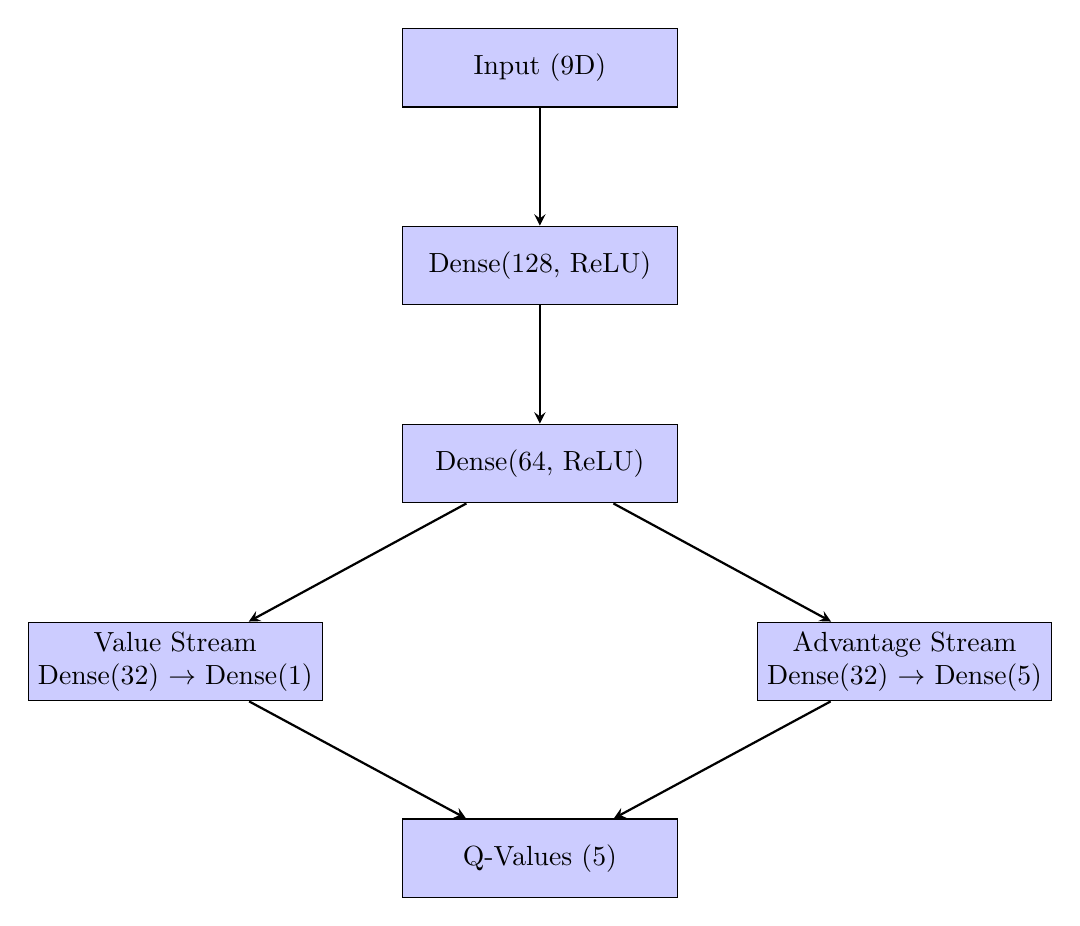
\begin{tikzpicture}[
    node distance=1.5cm,
    layer/.style={rectangle, draw, fill=blue!20, minimum width=3.5cm, minimum height=1cm, align=center},
    arrow/.style={thick,->,>=stealth}
]
    \node[layer] (input) {Input (9D)};
    \node[layer, below=of input] (fc1) {Dense(128, ReLU)};
    \node[layer, below=of fc1] (fc2) {Dense(64, ReLU)};
    
    \node[layer, below left=1.5cm and 1cm of fc2, text width=3.5cm] (value) {Value Stream\\Dense(32) $\rightarrow$ Dense(1)};
    \node[layer, below right=1.5cm and 1cm of fc2, text width=3.5cm] (adv) {Advantage Stream\\Dense(32) $\rightarrow$ Dense(5)};
    
    \node[layer, below=4cm of fc2] (output) {Q-Values (5)};
    
    \draw[arrow] (input) -- (fc1);
    \draw[arrow] (fc1) -- (fc2);
    \draw[arrow] (fc2) -- (value);
    \draw[arrow] (fc2) -- (adv);
    \draw[arrow] (value) -- (output);
    \draw[arrow] (adv) -- (output);
\end{tikzpicture}%
}
\caption{Dueling DQN Network Architecture showing the separation of value and advantage streams.}
\label{fig:dueling_arch}
\end{figure}

\subsection{Training Process}

We trained the agent for 1000 episodes, with each episode lasting up to 100 timesteps. The agent uses an epsilon-greedy policy---basically, it picks a random action with probability $\epsilon$ and the action its network thinks is best with probability $1 - \epsilon$. Epsilon starts at 1.0 (fully random) and decays exponentially with a factor of 0.995, eventually bottoming out at 0.01. The idea is simple: explore a lot early on to discover what works, then gradually shift to exploiting what you've learned.

We store every transition (state, action, reward, next state, done) in a replay buffer that holds up to 10,000 transitions. During training, we sample random minibatches of 64 from this buffer. Sampling randomly like this breaks the correlation between consecutive experiences, which is important because correlated samples can really destabilize neural network training. The target network, updated every 10 episodes, gives us stable training targets and prevents the kind of oscillation you'd get from chasing a moving target.

\subsubsection{Training Algorithm}

Algorithm \ref{alg:dqn_training} lays out the full training procedure. It's essentially the standard DQN loop with Double DQN target computation and periodic target network updates---nothing exotic, but the combination works well for our setting.

\begin{algorithm}[H]
\caption{DQN Training Loop}
\label{alg:dqn_training}
\begin{algorithmic}[1]
\State Initialize Q-network $Q_\theta$ with random weights
\State Initialize target network $Q_{\theta^-} \leftarrow Q_\theta$
\State Initialize replay buffer $\mathcal{D}$
\For{episode $= 1$ to $N$}
    \State Reset environment: $s_0 \leftarrow$ env.reset()
    \For{step $= 1$ to $T$}
        \State Select action: $a \leftarrow \epsilon\text{-greedy}(Q_\theta(s))$
        \State Execute action: $s', r, done \leftarrow$ env.step($a$)
        \State Store transition: $\mathcal{D} \leftarrow \mathcal{D} \cup \{(s, a, r, s', done)\}$
        \State Sample minibatch from $\mathcal{D}$
        \State Compute targets using Double DQN
        \State Update $Q_\theta$ via gradient descent
        \State $s \leftarrow s'$
        \If{done}
            \State \textbf{break}
        \EndIf
    \EndFor
    \State Decay $\epsilon$
    \If{episode mod 10 $= 0$}
        \State Update target network: $Q_{\theta^-} \leftarrow Q_\theta$
    \EndIf
\EndFor
\end{algorithmic}
\end{algorithm}

\subsubsection{Weight Update Formula}

For the weight updates, we use the Double DQN target formula. The target Q-value for a given transition is:

\begin{equation}
y_i = r_i + \gamma \cdot Q_{\theta^-}(s'_i, \arg\max_{a'} Q_\theta(s'_i, a')) \cdot (1 - d_i)
\end{equation}

Here, $r_i$ is the reward, $\gamma = 0.99$ is the discount factor, $s'_i$ is the next state, and $d_i$ indicates whether the episode ended. The important bit is that the online network $Q_\theta$ chooses which action looks best, but the target network $Q_{\theta^-}$ says how good that action actually is. This decoupling is what reduces the overestimation bias.

The loss is Huber loss computed over the minibatch:

\begin{equation}
\mathcal{L}(\theta) = \frac{1}{N} \sum_{i=1}^{N} L_\delta(Q_\theta(s_i, a_i) - y_i)
\end{equation}

And the weights get updated with Adam plus gradient clipping:

\begin{equation}
\theta \leftarrow \theta - \alpha \cdot \text{Adam}(\nabla_\theta \mathcal{L}(\theta))
\end{equation}

where $\alpha = 0.001$. We clip gradients to a max norm of 1.0 to keep things from blowing up during training.

\subsubsection{Loss Function}

We went with Huber loss (a.k.a. Smooth L1 loss), which is kind of a best-of-both-worlds choice. For small errors, it behaves like mean squared error (smooth, easy gradients). For large errors, it switches to something closer to absolute error, which is less sensitive to outliers. The definition is:

\begin{equation}
L_\delta(a) = \begin{cases} 
\frac{1}{2}a^2 & \text{if } |a| \leq \delta \\
\delta(|a| - \frac{1}{2}\delta) & \text{otherwise}
\end{cases}
\end{equation}

We used $\delta = 1.0$, and $a$ here is the TD error $Q_\theta(s, a) - y$. The practical benefit is that the occasional outlier experience doesn't cause a huge gradient spike that destabilizes the whole network.

\subsubsection{Epsilon-Greedy Schedule}

The exploration rate decays according to:

\begin{equation}
\epsilon_t = \max(\epsilon_{end}, \epsilon_{start} \times \epsilon_{decay}^t)
\end{equation}

With $\epsilon_{start} = 1.0$, $\epsilon_{end} = 0.01$, and $\epsilon_{decay} = 0.995$, the schedule looks like this:

\begin{table}[H]
\centering
\caption{Epsilon Decay Schedule}
\begin{tabular}{lcc}
\toprule
\textbf{Episode} & \textbf{Epsilon} & \textbf{Exploration Rate} \\
\midrule
0 & 1.00 & 100\% random \\
100 & 0.61 & 61\% random \\
200 & 0.37 & 37\% random \\
300 & 0.22 & 22\% random \\
500 & 0.08 & 8\% random \\
1000 & 0.01 & 1\% random \\
\bottomrule
\end{tabular}
\end{table}

So the agent is basically picking random actions for the first couple hundred episodes, but by episode 500 it's mostly relying on what it's learned.

%==============================================================================
\section{Baseline Agents}
%==============================================================================

\subsection{Random Agent}

This is our lower bound---an agent that just picks an action at random each timestep, with no knowledge of what's going on. Obviously nobody would deploy this in practice, but it's useful as a sanity check. Any agent that can't comfortably beat the random baseline hasn't really learned anything.

\subsection{Threshold Agent}

The threshold agent uses fixed cutoffs on the observable metrics to decide what to do. This is actually pretty close to how a lot of basic SIEM alert rules work in the real world. If the login rate exceeds 50 and the file rate is above 100, it goes straight to host isolation. If just the login rate is high, it locks the account. Moderate login elevation triggers an IP block. Elevated file access triggers process termination. Otherwise, it does nothing.

It's simple, but it captures the basic logic of many deployed systems, which makes it a useful comparison point.

\subsection{Snort-Inspired Agent}

We modeled this baseline on the kind of thresholding rules you'd find in a Snort deployment. It has an SSH brute force threshold of 10 login attempts (low-level alert) and 30 attempts (critical response), and it detects ransomware-like behavior from combinations of rapid file access and CPU anomalies. It's not real packet inspection, obviously---we're working with metric thresholds---but it captures the conceptual approach of signature-based detection.

\subsection{NIST 800-61 Agent}

This one follows the NIST incident handling guidelines. It computes a weighted impact score from the three observable metrics (login and file access weighted at 0.4 each, CPU at 0.2) and then picks a response based on how severe the computed impact is. High impact (score above 0.8) triggers immediate isolation; lower scores get less aggressive responses, in line with NIST's incident categorization approach.

\subsection{MITRE ATT\&CK Agent}

The MITRE baseline tries to match observable patterns to specific ATT\&CK techniques. High login rates trigger detection of T1110 (Brute Force), with even higher rates mapping to T1110.001 (Password Guessing). Combined file access and CPU anomalies trigger T1486 (Data Encrypted for Impact), which is the ransomware technique. The response severity scales with the most serious technique detected.

This is a simplified version of what a real ATT\&CK-based detection system would look like, but it captures the idea of mapping observed behavior to known adversary techniques and responding accordingly.

%==============================================================================
\section{Experimental Results}
%==============================================================================

\subsection{Training Performance}

We trained for 1000 episodes using the setup described in Section 3. The learning curve (Figure \ref{fig:learning_curve}) shows the kind of pattern you'd expect from DQN training: the agent starts off doing pretty badly while it's mostly exploring, then gradually improves as it starts to figure out what works.

\begin{figure}[H]
\centering
\includegraphics[width=0.9\textwidth]{figures/learning_curve.png}
\caption{Learning curve showing episode rewards over 1000 training episodes. The moving average (orange line) shows steady improvement from negative rewards early on to positive rewards in later episodes.}
\label{fig:learning_curve}
\end{figure}

In the first 100 episodes or so, the agent averaged around $-200$ in reward---epsilon was still high, so it was mostly taking random actions and suffering the consequences. By episodes 301--500, the mean reward had climbed to roughly +15, meaning the agent was starting to recognize attacks and respond to them appropriately. In the final 200 episodes, rewards stabilized around +20 to +40, with the policy continuing to get a bit better but mostly converged.

\begin{figure}[H]
\centering
\includegraphics[width=0.9\textwidth]{figures/epsilon_decay.png}
\caption{Epsilon decay over training episodes, showing the transition from exploration (high epsilon) to exploitation (low epsilon).}
\label{fig:epsilon_decay}
\end{figure}

Figure \ref{fig:epsilon_decay} shows how epsilon decayed over the course of training. The exponential decay brings it below 0.1 by around episode 500, and it settles at the floor of 0.01.

\begin{figure}[H]
\centering
\includegraphics[width=0.9\textwidth]{figures/loss_curve.png}
\caption{Training loss over episodes, showing initial instability followed by convergence as the Q-network learns to predict action values more accurately.}
\label{fig:loss_curve}
\end{figure}

The loss curve (Figure \ref{fig:loss_curve}) shows the TD error going down over training, as you'd hope. It starts high because the network's predictions are basically random at first, then drops as it gets better at estimating Q-values. There's some wobbling in the later stages, which is normal---it happens when the target network updates and the targets shift a bit.

\subsection{Final Training Statistics}

Training took about 28--30 minutes on our setup (nothing fancy, just a standard computing environment). The best single episode hit a reward of 234.0, which happened when the agent caught multiple attacks early. The worst episode was $-812.0$---a case where it missed an attack that went all the way to compromise. The average reward over the last 100 episodes settled at 20.23, which we take as a sign of stable, converged performance.

Over the entire training run, the agent contained 856 attacks and generated 11,193 false positives. That false positive number looks bad, but it's heavily skewed by the early exploration phase where the agent was basically mashing random buttons. The rate drops off substantially once epsilon decays and the agent starts making more informed decisions. Final epsilon reached the minimum of 0.01.

\begin{figure}[H]
\centering
\includegraphics[width=0.9\textwidth]{figures/performance_metrics.png}
\caption{Performance metrics over training showing attacks contained, false positives, and success rate evolution.}
\label{fig:performance_metrics}
\end{figure}

\subsection{Final Evaluation Results}

For the final evaluation, we ran the trained agent for 100 episodes with epsilon fixed at 0.01 (essentially pure exploitation, with just a tiny bit of random exploration). The average reward was 40.15 with a standard deviation of 65.40. The success rate---meaning episodes that ended without the system being compromised---came in at 75.0\%. On average, the agent triggered 0.55 false positives per episode while containing 0.88 attacks per episode. That ratio (far more attacks contained than false alarms generated) suggests the agent has learned to discriminate between actual threats and normal fluctuations reasonably well.

\begin{figure}[H]
\centering
\includegraphics[width=0.9\textwidth]{figures/reward_distribution.png}
\caption{Distribution of episode rewards in final evaluation. The bimodal shape corresponds to successful defense (positive cluster) and missed attacks (negative tail).}
\label{fig:reward_distribution}
\end{figure}

The reward distribution in Figure \ref{fig:reward_distribution} has a somewhat bimodal shape. There's a cluster of positive rewards from episodes where the agent successfully defended against attacks, and a tail of negative rewards from episodes where attacks made it through.

\subsection{Baseline Comparison}

We ran all the baseline agents through the same 100 episodes, using identical random seeds to keep the comparison fair. Table \ref{tab:baseline_comparison} has the full results.

\begin{table}[H]
\centering
\caption{Agent Comparison Results from Final Evaluation}
\label{tab:baseline_comparison}
\begin{tabular}{lrr}
\toprule
\textbf{Agent} & \textbf{Average Reward} & \textbf{Standard Deviation} \\
\midrule
DQN (Ours) & \textbf{34.33} & 73.63 \\
NIST 800-61 & 11.90 & 67.18 \\
Threshold & 10.37 & 63.27 \\
MITRE ATT\&CK & 7.48 & 60.69 \\
Do-Nothing & 2.45 & 64.99 \\
Snort-Inspired & -2.08 & 60.29 \\
Random & -644.31 & 155.65 \\
\bottomrule
\end{tabular}
\end{table}

The DQN agent came out on top across the board. The gap against the random baseline is enormous (about 679 reward points), which at minimum confirms the agent learned something real. More interesting is that it also beat all the structured baselines---the NIST-inspired agent came second, followed closely by the threshold agent, with the MITRE and Snort baselines further back. The do-nothing agent actually managed a slightly positive average, which makes sense given that attacks don't happen every episode and the correct action during quiet periods is literally to do nothing.

\begin{figure}[H]
\centering
\includegraphics[width=0.8\textwidth]{figures/action_preferences.png}
\caption{Action preferences learned by the DQN agent during evaluation.}
\label{fig:action_preferences}
\end{figure}

Looking at what actions the agent actually took (Figure \ref{fig:action_preferences}), there's a clear pattern: it favors less aggressive responses when observations are within normal ranges, and ramps up to more severe actions when attack indicators are present. This suggests it's learned a context-sensitive policy rather than just defaulting to one action all the time.

\subsection{Statistical Significance Testing}

We wanted to make sure these results weren't just noise, so we ran the standard battery of statistical tests. For each DQN-vs-baseline comparison, we did an independent samples t-test, computed Cohen's d for effect size, and constructed 95\% confidence intervals.

\begin{table}[H]
\centering
\caption{Statistical Significance Tests (DQN vs All Baselines)}
\label{tab:stats_tests}
\begin{tabular}{lrrrcc}
\toprule
\textbf{Comparison} & \textbf{T-statistic} & \textbf{P-value} & \textbf{Cohen's d} & \textbf{95\% CI} & \textbf{Significant} \\
\midrule
DQN vs Random & 39.21 & <0.001 & 5.55 & [644.51, 712.76] & $\checkmark$ \\
DQN vs Snort & 3.81 & <0.001 & 0.54 & [17.55, 55.27] & $\checkmark$ \\
DQN vs Do-Nothing & 3.23 & 0.001 & 0.46 & [12.42, 51.34] & $\checkmark$ \\
DQN vs MITRE & 2.80 & 0.006 & 0.40 & [7.93, 45.76] & $\checkmark$ \\
DQN vs Threshold & 2.46 & 0.015 & 0.35 & [4.71, 43.19] & $\checkmark$ \\
DQN vs NIST & 2.24 & 0.026 & 0.32 & [2.67, 42.18] & $\checkmark$ \\
\bottomrule
\end{tabular}
\end{table}

Every comparison came back statistically significant at $p < 0.05$. The effect sizes tell a useful story. Against the random baseline, Cohen's d is 5.55---which is huge by any standard, confirming that the agent has learned genuinely useful behavior. Against the Snort baseline, $d = 0.54$ is a medium effect, suggesting the learned policy picks up on things that fixed threshold rules miss.

The effect sizes against the stronger baselines (threshold, NIST, MITRE) range from 0.32 to 0.40---smaller, but still meaningful. In practical terms, even the tightest comparison (DQN vs NIST, $d = 0.32$) has a confidence interval of [2.67, 42.18] that excludes zero, so we can be fairly confident the DQN is genuinely better, not just lucky.

\subsection{Training Improvement Analysis}

As a final check that the agent actually learned over the course of training (rather than just getting lucky near the end), we compared rewards from the first half (episodes 1--500) against the second half (episodes 501--1000). The first-half mean was $-165.90$, reflecting all that early random exploration. The second-half mean was $18.67$. That's a difference of about 185 reward points, which is highly significant ($t = 20.81$, $p < 0.001$, Cohen's $d = 1.32$). The 95\% confidence interval of [167.16, 201.97] for the improvement is comfortably far from zero.

%==============================================================================
\section{Discussion}
%==============================================================================

\subsection{Key Findings}

The main takeaway from our experiments is that DRL can learn incident response policies that outperform traditional rule-based approaches, at least in our simulated setting. The DQN agent beat every baseline we tested, and the improvements held up under statistical scrutiny.

The Dueling architecture seemed to help quite a bit here. By separating the estimation of ``how good is this state?'' from ``how much does my action choice matter?,'' the network can handle states where the right action is obvious (everything's fine, do nothing) without that confusing the learning in states where the decision is actually hard (is this an attack starting or just a spike in legitimate activity?). That fits the structure of the incident response problem nicely.

The 9-dimensional observation space also pulled its weight. The rate-of-change features were particularly useful for catching the sudden jumps that come with attack onset, while the moving averages helped the agent distinguish sustained anomalies (likely attacks) from brief legitimate spikes. The sustained anomaly indicator added temporal context that you just can't get from looking at a single point in time.

\subsection{Comparison with Threshold Baseline}

It's worth spending a moment on the fact that the effect size against the threshold baseline was relatively modest ($d = 0.35$). In some ways this isn't surprising---for the attack patterns in our simulation, reasonably well-chosen thresholds can do an okay job. So where's the value of the RL approach?

A few places, we think. First, the RL agent figured out its own ``thresholds'' from data, without us having to hand-tune anything. In a real deployment, getting those thresholds right is a nontrivial exercise that requires domain expertise and constant adjustment. Second, the agent can learn temporal patterns and action sequences that simple threshold rules just can't express---for instance, it might learn that a moderate spike followed by a sustained elevation warrants a different response than a single sharp spike that quickly subsides. Third, the learned policy could in principle be retrained as attack patterns change, whereas rule-based systems need manual updates.

We should also acknowledge that our threshold baseline is quite simplified. A real-world SIEM would use many more features, more sophisticated correlation rules, and probably some machine learning on top. The comparison gives us a useful signal but shouldn't be over-interpreted.

\subsection{Limitations}

We want to be upfront about the limitations of this work. The most obvious one is that we're working in simulation, not the real world. Our environment, while based on real dataset parameters, is still a simplified model of what actual attacks look like. Deploying something like this in production would involve a whole set of additional challenges: integrating with existing security infrastructure, handling a much wider and more sophisticated range of attacks, dealing with adversaries who might actively try to evade the agent, and figuring out how much autonomy to give an automated system versus keeping a human in the loop.

Our baselines, too, are simplifications. Real Snort deployments do deep packet inspection, not just metric thresholding. NIST 800-61 in practice involves human judgment and documentation that our automated version doesn't capture. And a proper MITRE ATT\&CK detection system would use specific indicators of compromise, not just behavioral metrics.

There's also the variance issue with RL training. Different random seeds can lead to noticeably different policies, and we only ran a single training run. Running the whole thing multiple times and reporting aggregate statistics would make the conclusions more robust. That's something we'd want to do in a more thorough study.

\subsection{Practical Implications}

For anyone thinking about using RL for incident response in practice, a few things stand out from our work. The big improvement over random and do-nothing baselines confirms that RL can learn meaningful defensive behavior---it's not just memorizing or getting lucky. The improvements over structured baselines suggest there's value beyond what simple rules can capture, though the magnitude depends on how good your rules already are.

That said, we wouldn't recommend giving an RL agent full autonomous control right out of the gate. A more realistic deployment would probably start with the agent making recommendations that a human analyst reviews and approves. Over time, as confidence in the system grows, lower-risk actions could be automated while higher-risk ones (like isolating a production server) stay under human control.

Retraining would also be important. Attack patterns change, and a policy that works great today might not be appropriate six months from now. The nice thing is that the same training infrastructure we used initially can support ongoing adaptation, potentially with a lower learning rate to avoid forgetting what the agent already knows while still picking up on new patterns.

%==============================================================================
\section{Conclusion}
%==============================================================================

In this project, we set out to see whether Deep Reinforcement Learning could be a viable approach for automated cybersecurity incident response. Motivated by the work of Hammar and Stadler \cite{hammar2021}, who demonstrated that DQN variants can learn effective cyber defense strategies in simulated environments, we built a custom Gymnasium environment that simulates brute force and ransomware attacks using Finite State Machines, with parameters drawn from the CICIDS 2017 and CERT datasets to keep the scenarios grounded in real data. We trained a Dueling Double DQN agent in this environment and then evaluated it against baselines inspired by Snort, NIST 800-61, and MITRE ATT\&CK.

The results are encouraging. The agent achieved a 75\% success rate and statistically significant improvements over every baseline, with Cohen's d ranging from 0.32 (against NIST rules) to 5.55 (against random). The statistical validation---t-tests, effect sizes, confidence intervals---gives us reasonable confidence that these aren't just flukes. Where \cite{hammar2021} focused on abstract network defense games, our results suggest the same family of algorithms can work for the more practical problem of choosing specific incident response actions from noisy system metrics.

There's plenty of room for future work, of course. More diverse attack scenarios, multi-agent settings, adversarial robustness testing, and eventually real-world deployment trials would all be natural next steps. Combining the self-play approach from \cite{hammar2021} with our dataset-driven simulation could also be interesting---training the agent against an adaptive adversary rather than fixed attack patterns. But as a proof of concept, we think the results make a decent case that RL-based incident response is worth pursuing further.

%==============================================================================
\section*{Acknowledgments}
%==============================================================================

We'd like to thank the creators of the CICIDS 2017 and CERT Insider Threat datasets for making their data publicly available. Without those resources, calibrating our attack simulations to realistic parameters would have been much harder.

%==============================================================================
\begin{thebibliography}{99}
%==============================================================================

\bibitem{mnih2015} Mnih, V., et al. (2015). Human-level control through deep reinforcement learning. \textit{Nature}, 518(7540), 529-533.

\bibitem{wang2016} Wang, Z., et al. (2016). Dueling network architectures for deep reinforcement learning. In \textit{ICML} (pp. 1995-2003).

\bibitem{hasselt2016} Van Hasselt, H., et al. (2016). Deep reinforcement learning with double Q-learning. In \textit{AAAI} (Vol. 30, No. 1).

\bibitem{cicids2017} Sharafaldin, I., et al. (2018). Toward generating a new intrusion detection dataset and intrusion traffic characterization. In \textit{ICISSP} (pp. 108-116).

\bibitem{cert} Glasser, J., \& Lindauer, B. (2013). Bridging the gap: A pragmatic approach to generating insider threat data. In \textit{IEEE Security and Privacy Workshops} (pp. 98-104).

\bibitem{nist80061} Cichonski, P., et al. (2012). Computer security incident handling guide. \textit{NIST Special Publication}, 800-61.

\bibitem{mitre} MITRE Corporation. (2021). MITRE ATT\&CK Framework. Retrieved from https://attack.mitre.org/

\bibitem{snort} Roesch, M. (1999). Snort: Lightweight intrusion detection for networks. In \textit{Lisa} (Vol. 99, No. 1, pp. 229-238).

\bibitem{gymnasium} Towers, M., et al. (2023). Gymnasium. GitHub repository.

\bibitem{tensorflow} Abadi, M., et al. (2016). TensorFlow: A system for large-scale machine learning. In \textit{OSDI} (Vol. 16, pp. 265-283).

\bibitem{hammar2021} Hammar, K., \& Stadler, R. (2021). Finding effective security strategies through reinforcement learning and self-play. In \textit{IEEE International Conference on Network and Service Management (CNSM)} (pp. 113-121). IEEE.

\end{thebibliography}

%==============================================================================
\appendix
\section{Implementation Details}
%==============================================================================

\subsection{Source Code}

All the code for this project is on GitHub:

\begin{center}
\projecturl
\end{center}

\subsection{Project Folder Structure}

\begin{lstlisting}[language=bash,caption=Project Directory Structure]
automated-incident-response-using-RL/
|-- main.py                    # CLI entry point
|-- requirements.txt           # Python dependencies
|-- extracted_params.json      # Dataset-derived parameters
|-- README.md                  # Project documentation
|
|-- src/
|   |-- config.py              # Configuration dataclasses
|   |-- preprocess.py          # Data preprocessing
|   |-- attack_simulator.py    # FSM-based attack models
|   |-- incident_env.py        # Gymnasium environment
|   |-- agent.py               # DQN agent implementation
|   |-- train.py               # Training loop
|   |-- evaluate.py            # Evaluation & visualization
|
|-- models/
|   |-- best_model.h5          # Best trained model weights
|   |-- best_model_metadata.json
|
|-- logs/
|   |-- training_metrics.json  # Training history
|   |-- baseline_comparison.json
|
|-- figures/
|   |-- learning_curve.png
|   |-- epsilon_decay.png
|   |-- loss_curve.png
|   |-- performance_metrics.png
|   |-- reward_distribution.png
|   |-- action_preferences.png
|   |-- q_value_heatmap.png
|
|-- data/                      # Dataset files (not included)
    |-- CICIDS2017/
    |-- CERT/
\end{lstlisting}

\subsection{Requirements}

You'll need the following Python packages:

\begin{lstlisting}[caption=requirements.txt]
tensorflow>=2.10.0
numpy>=1.21.0
pandas>=1.3.0
gymnasium>=0.28.0
scipy>=1.7.0
tqdm>=4.62.0
matplotlib>=3.4.0
seaborn>=0.11.0
\end{lstlisting}

Install everything with:
\begin{lstlisting}[language=bash]
pip install -r requirements.txt
\end{lstlisting}

\subsection{Commands}

\subsubsection{Training}

To train the DQN agent:
\begin{lstlisting}[language=bash]
# Basic training (1000 episodes)
python main.py train --episodes 1000

# Training with baseline comparison
python main.py train --episodes 1000 --compare-baselines

# Training with N-step returns
python main.py train --episodes 1000 --n-step --n-steps 3

# Training with prioritized replay
python main.py train --episodes 1000 --prioritized-replay
\end{lstlisting}

\subsubsection{Preprocessing}

To preprocess the datasets and extract attack parameters:
\begin{lstlisting}[language=bash]
python main.py preprocess
\end{lstlisting}

\subsubsection{Output Files}

After training finishes, you'll find these output files:

\begin{table}[H]
\centering
\caption{Training Output Files}
\begin{tabular}{ll}
\toprule
\textbf{Path} & \textbf{Description} \\
\midrule
models/best\_model.h5 & Best trained model weights \\
logs/training\_metrics.json & Episode rewards, losses, epsilon \\
logs/baseline\_comparison.json & Statistical test results \\
figures/*.png & Visualization plots \\
\bottomrule
\end{tabular}
\end{table}

\end{document}